%!TEX root = minta_dolgozat.tex
%%%%%%%%%%%%%%%%%%%%%%%%%%%%%%%%%%%%%%%%%%%%%%%%%%%%%%%%%%%%%%%%%%%%%%%
\chapter{User documentation}\label{ch:BASIC}
%%%%%%%%%%%%%%%%%%%%%%%%%%%%%%%%%%%%%%%%%%%%%%%%%%%%%%%%%%%%%%%%%%%%%%%

\begin{summary}
	In this chapter E-me is described from a user point of view.
\end{summary}

%%%%%%%%%%%%%%%%%%%%%%%%%%%%%%%%%%%%%%%%%%%%%%%%%%%%%%%%%%%%%%%%%%%%%%%
The building blocks of E-me are pages.
The primary role of these pages is allowing the user to manage their PDF documents that were created through the application.
This management includes the ability to request a new document, view already owned documents, make modifications to them, delete the ones that are
obsolete or contain incorrect data, or even share them with other devices using a QR code.

The secondary role is collecting the data from the user that is necessary for generating their documents. 
This data is then encrypted, processed and later on added to the documents that the user requests. 

	\section{Introductory Pages}

		For an unauthenticated user there are 3 pages available in the application: Greeting, Login and Registration pages.
		Upon opening the application, the user is confronted with the Greeting page which allows them to navigate to the Login and Registration pages using the dedicated buttons.

		The Registration page consists of five text fields.
		Each of these fields are required in order to create a new user, however only two of them are needed for authentication: Login name and Password.
		The restrictions for these fields are the following:
		\begin{itemize}
			\item The Email and Login Name fields should be unique.
			\item The Password and Confirm password fields should be identical.
			\item The Email field should be a valid email address.
		\end{itemize}
		
		Upon successful registration, the application navigates the user to the Login Page in order for them to authenticate themselves using the Login Name and Password they entered.
		If the authentication was successful, the main shell appears where three tabs can be seen: My Documents, Request Document and Personal Info.

		\begin{figure}[H]
			\centering
			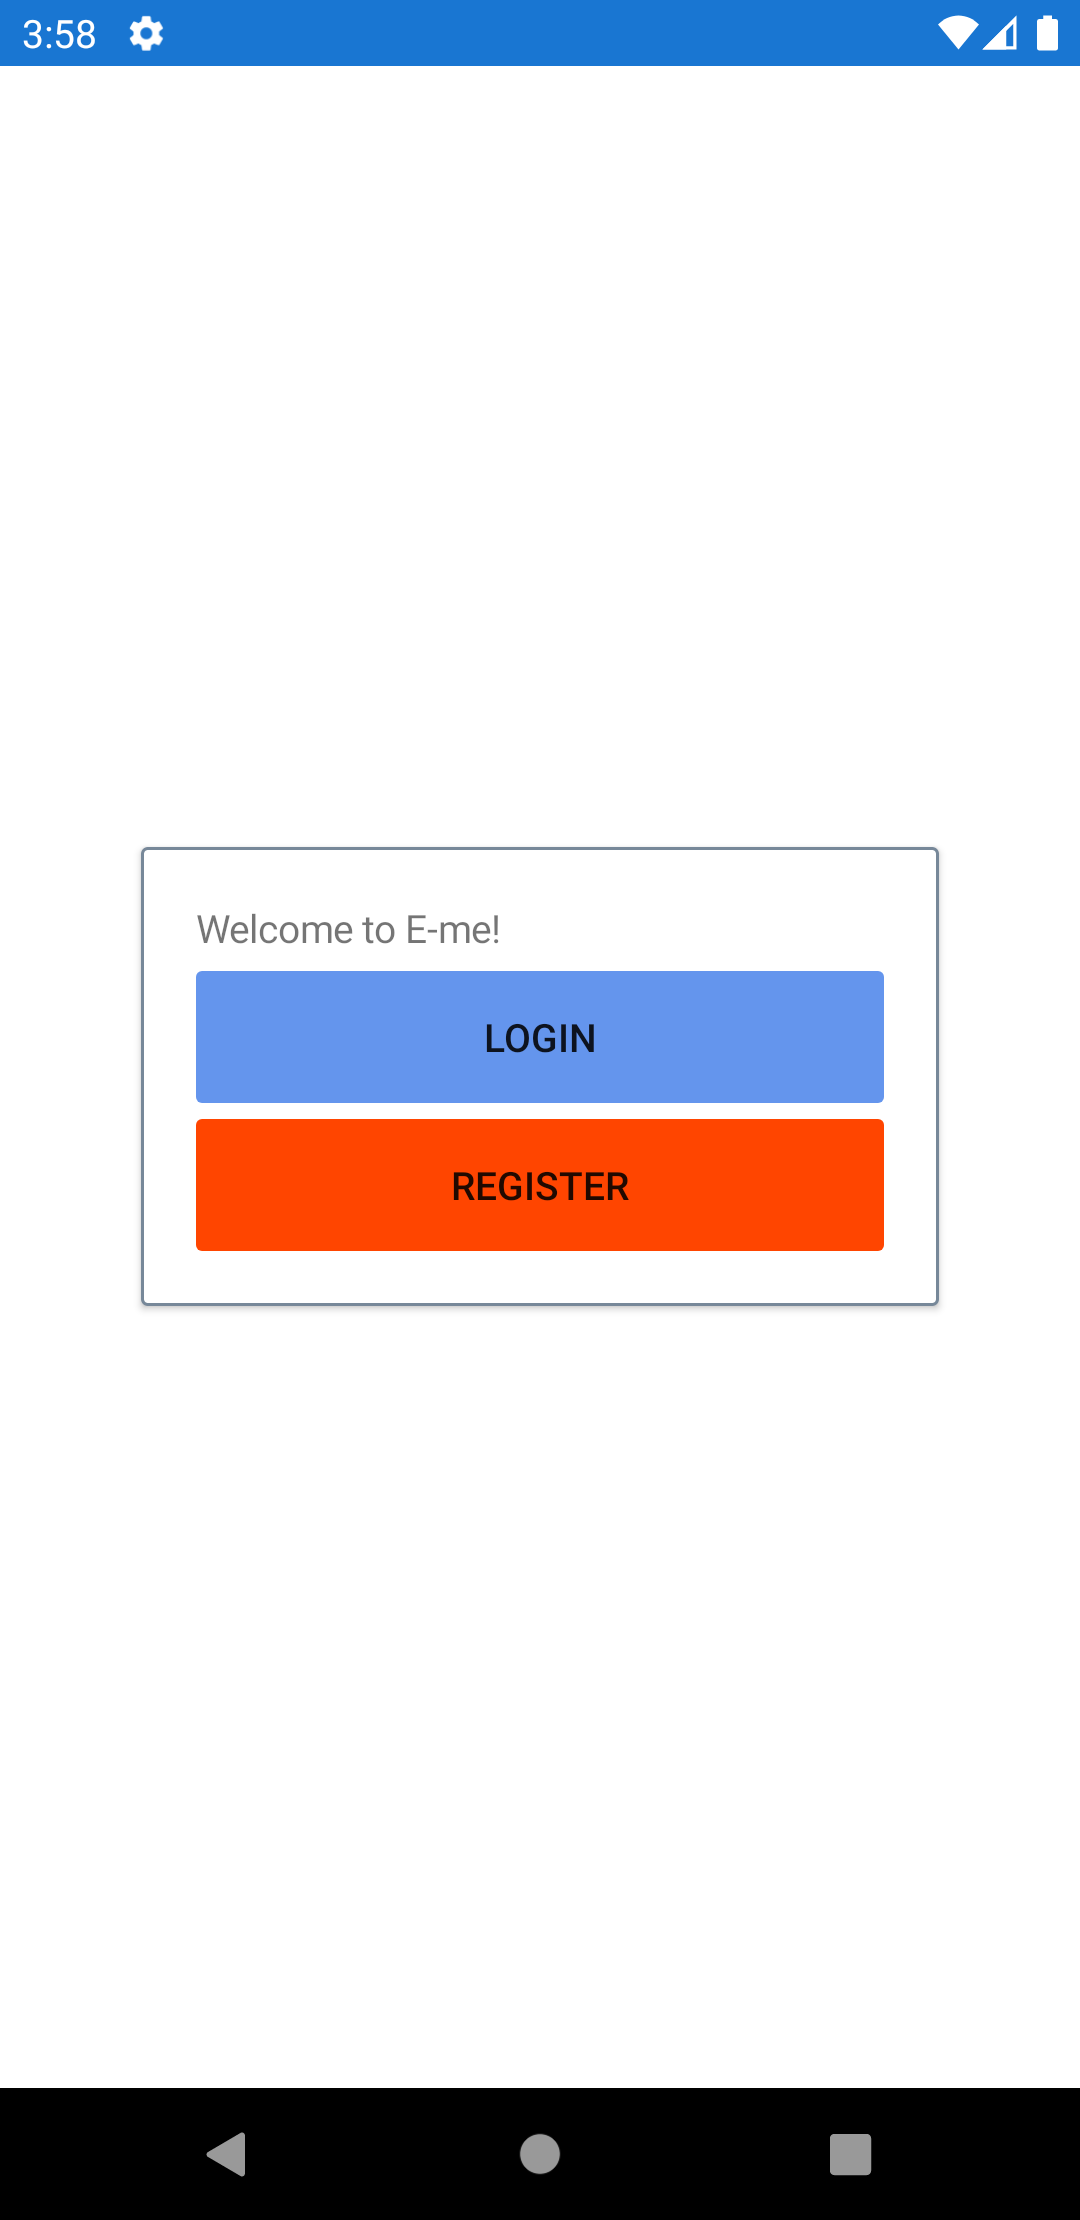
\includegraphics[scale=0.12]{main-page}				
			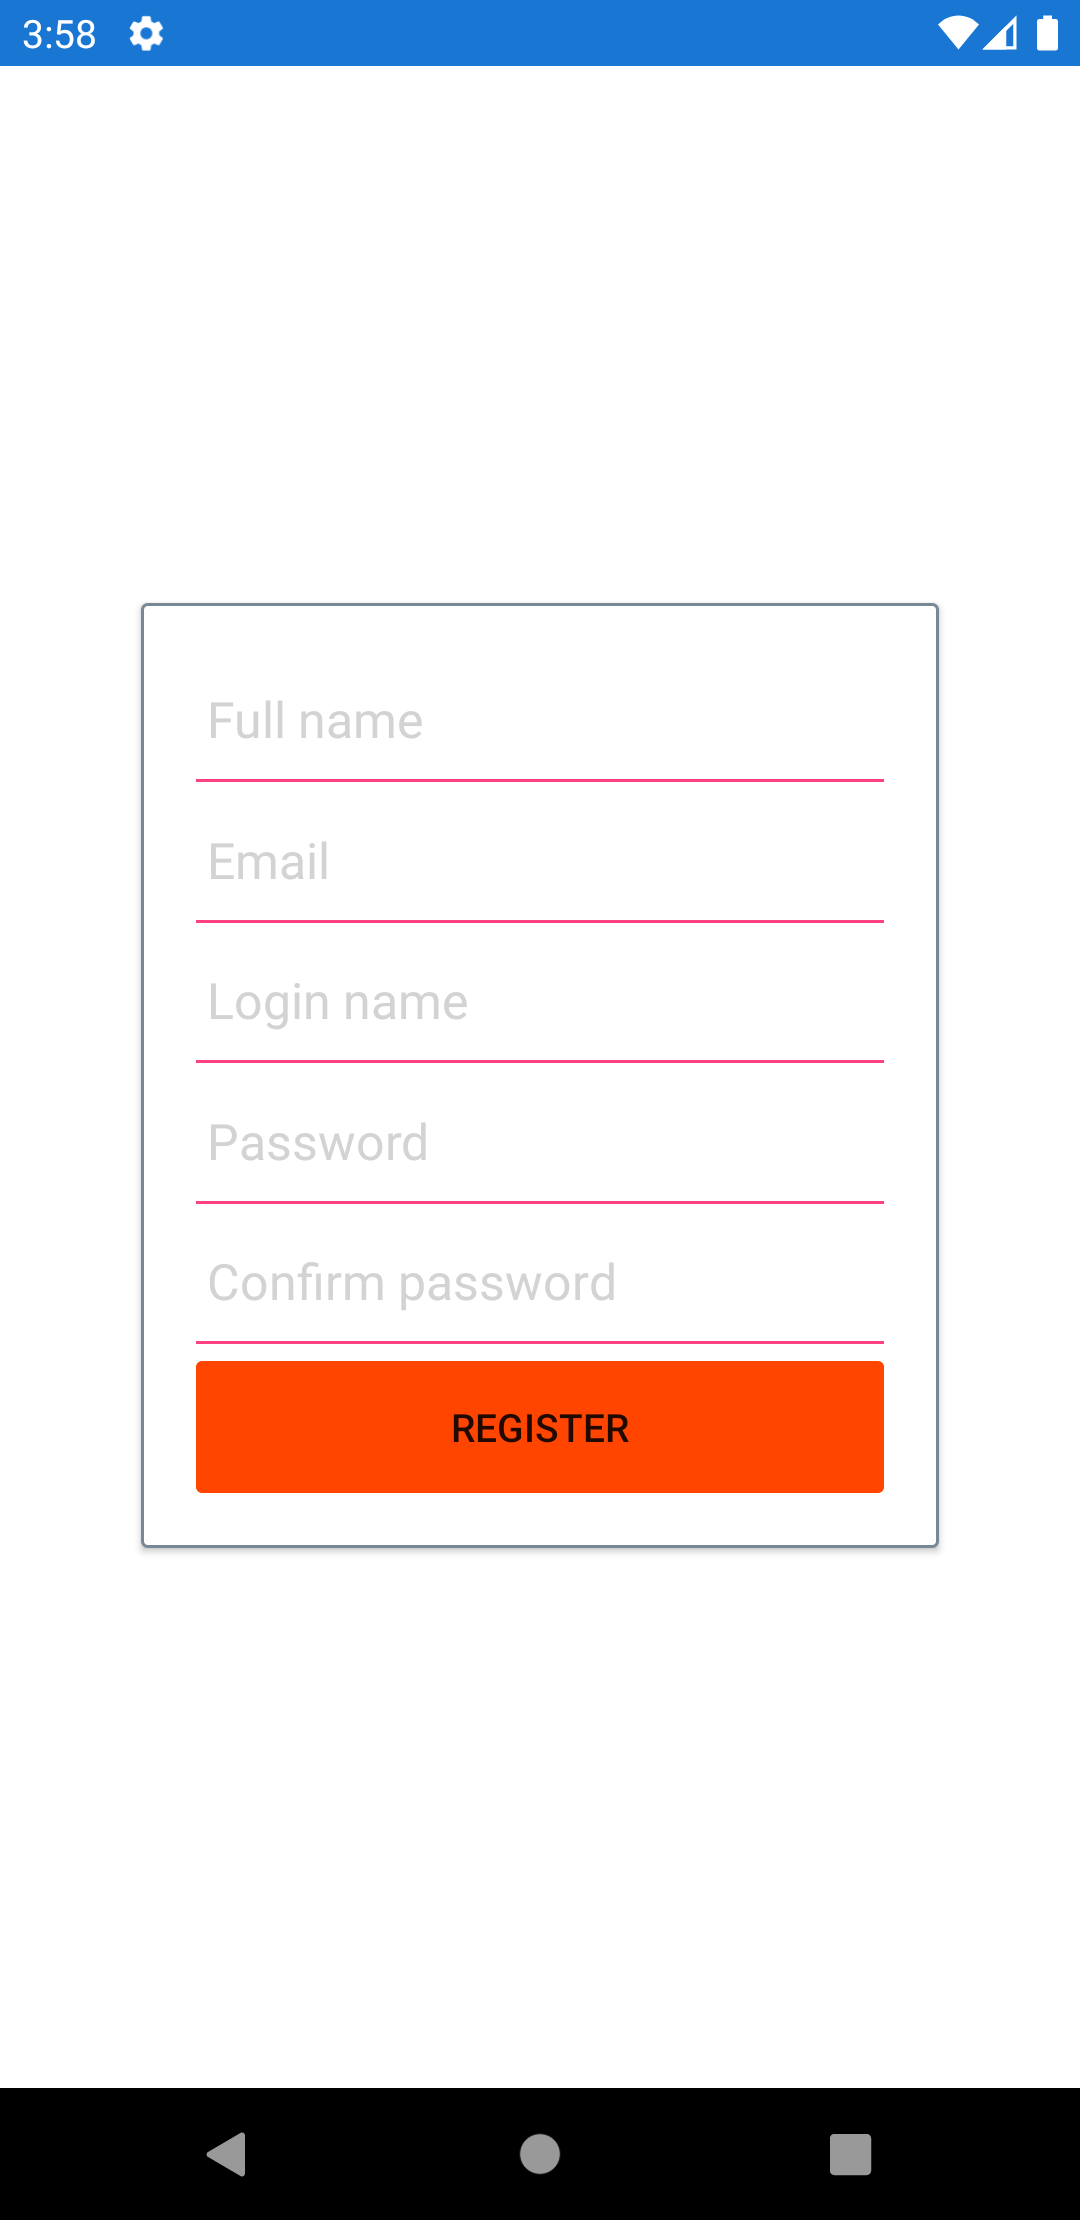
\includegraphics[scale=0.12]{register-page}			
			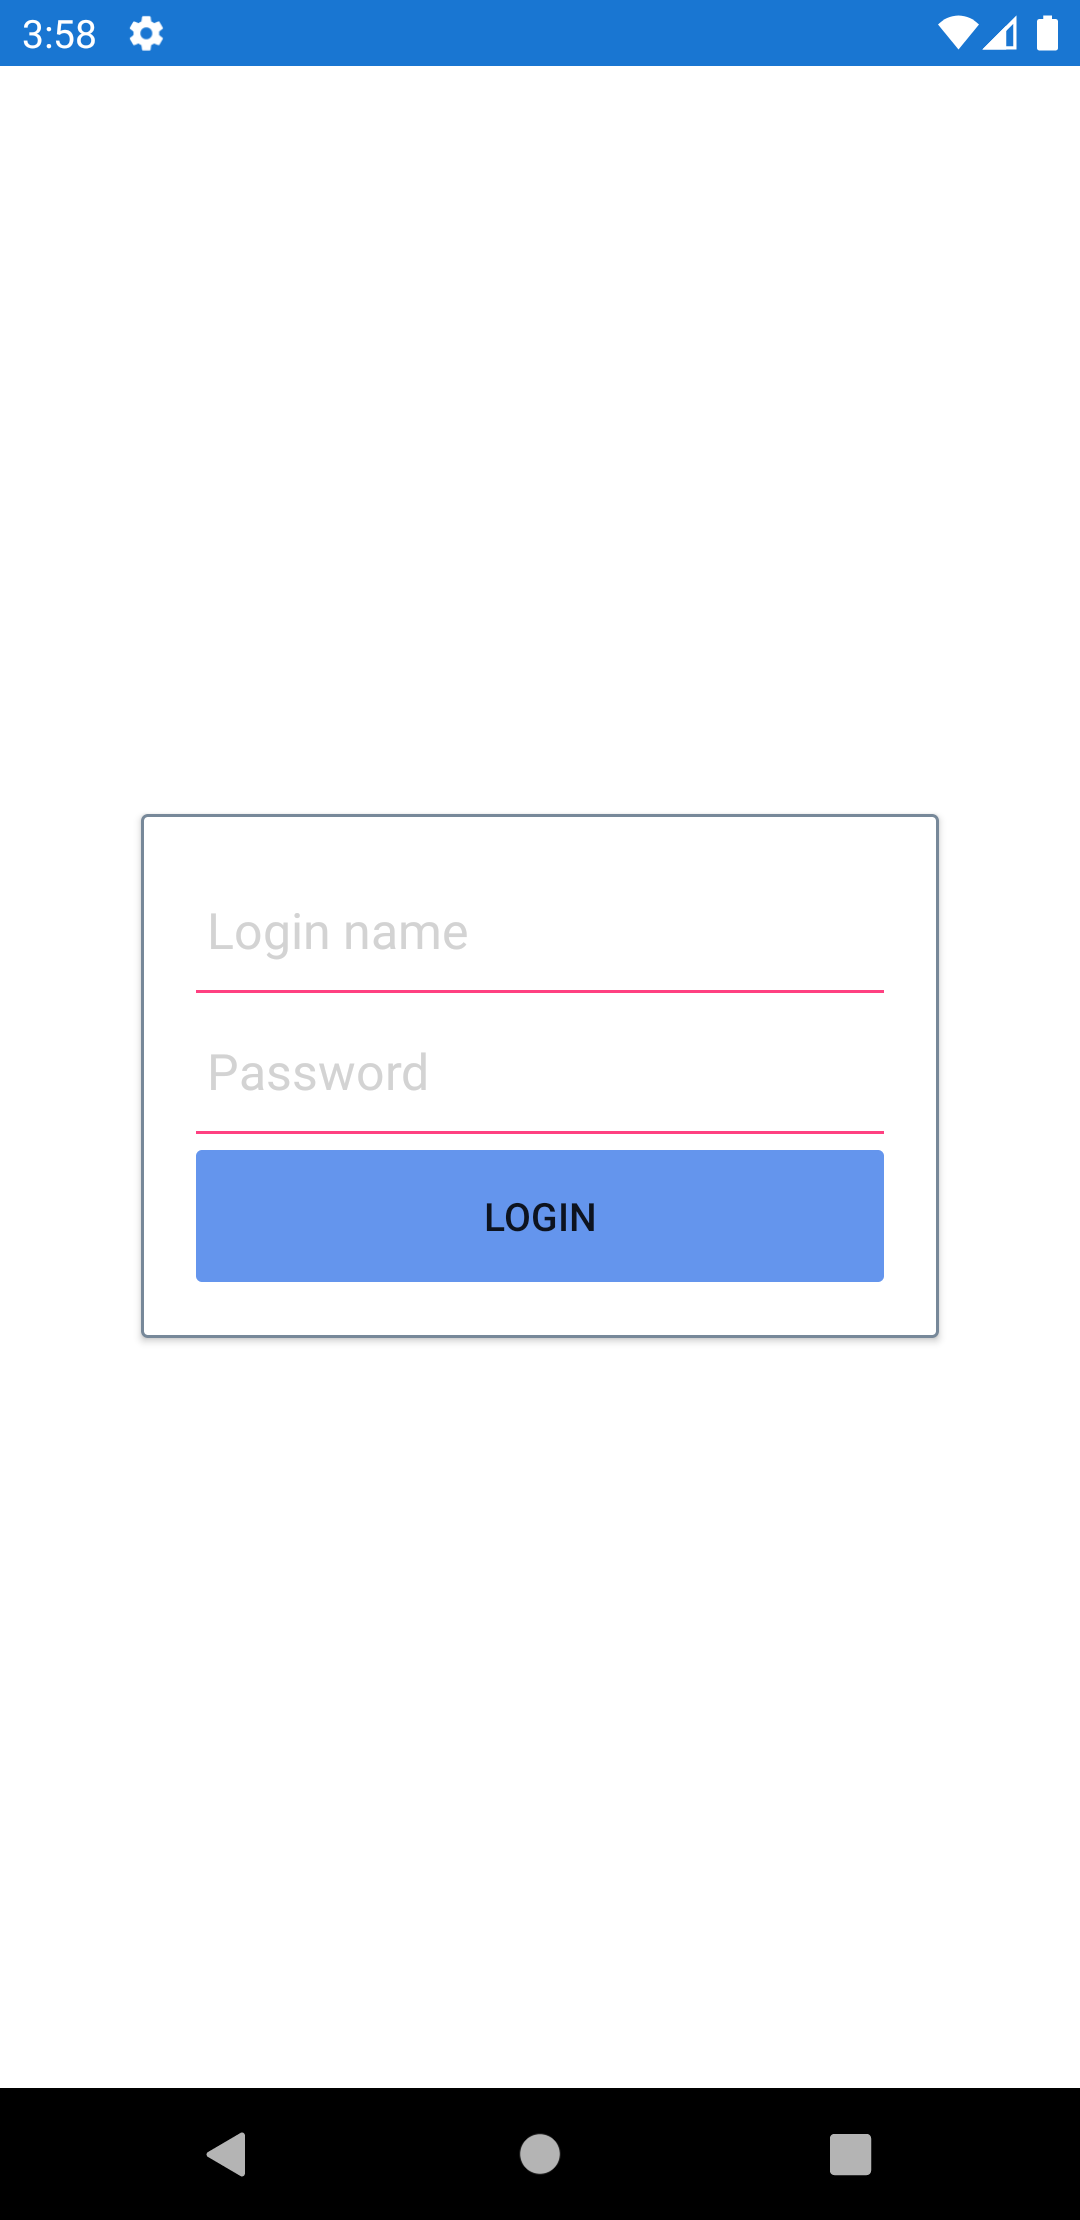
\includegraphics[scale=0.12]{login-page}				
			\caption{Introductory pages (Greeting, Registration, Login)}
		\end{figure}

	\section{My Documents}\label{documents}
	The My Documents page consists of two main parts: the list of documents and the "Scan QR code" button.
	The list of documents allows the user to visualize what types of documents they own.
	On each document two actions can be performed: Share and Remove.

		\begin{figure}[H]
			\centering
			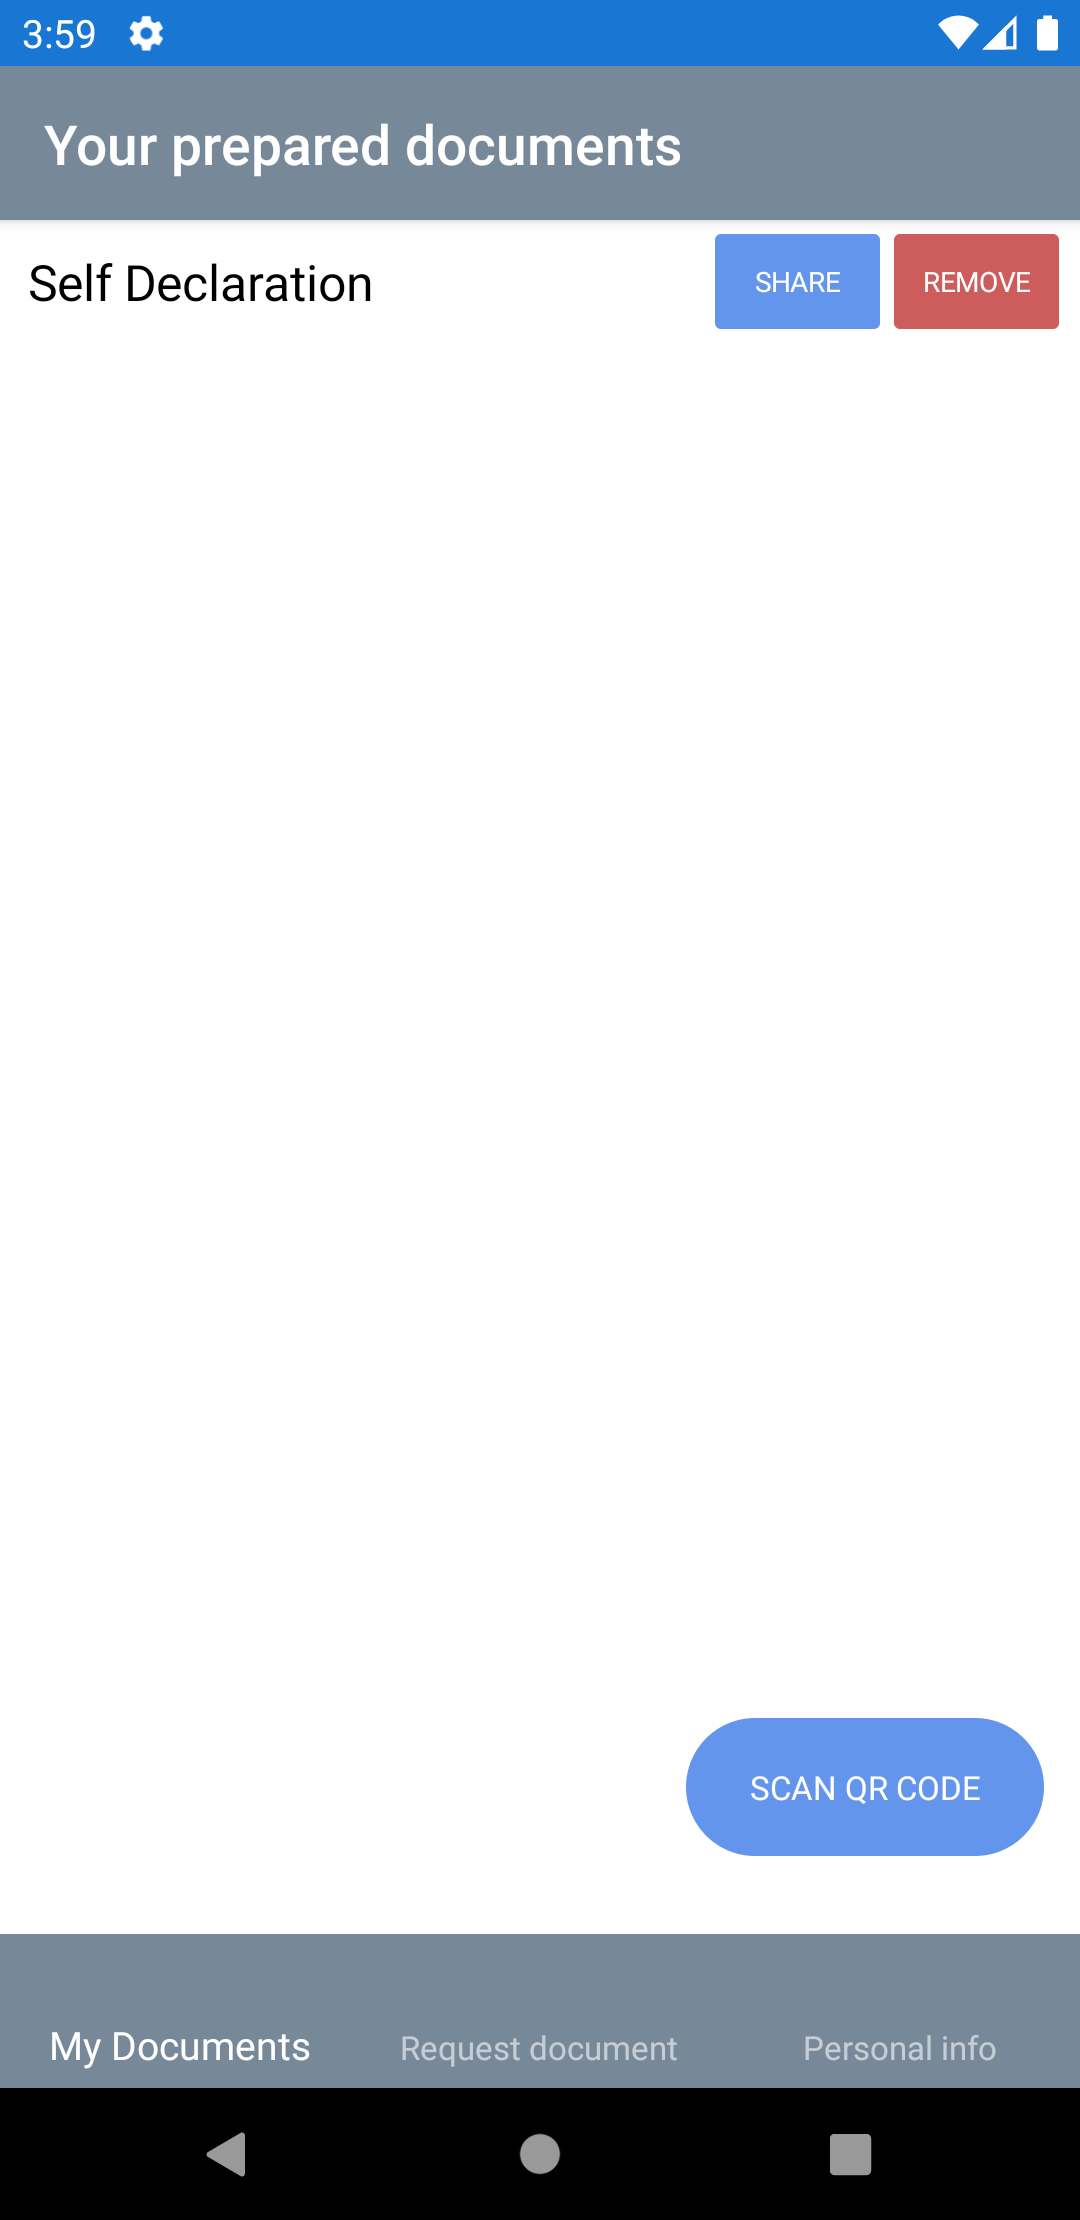
\includegraphics[scale=0.12]{documents-page}				
			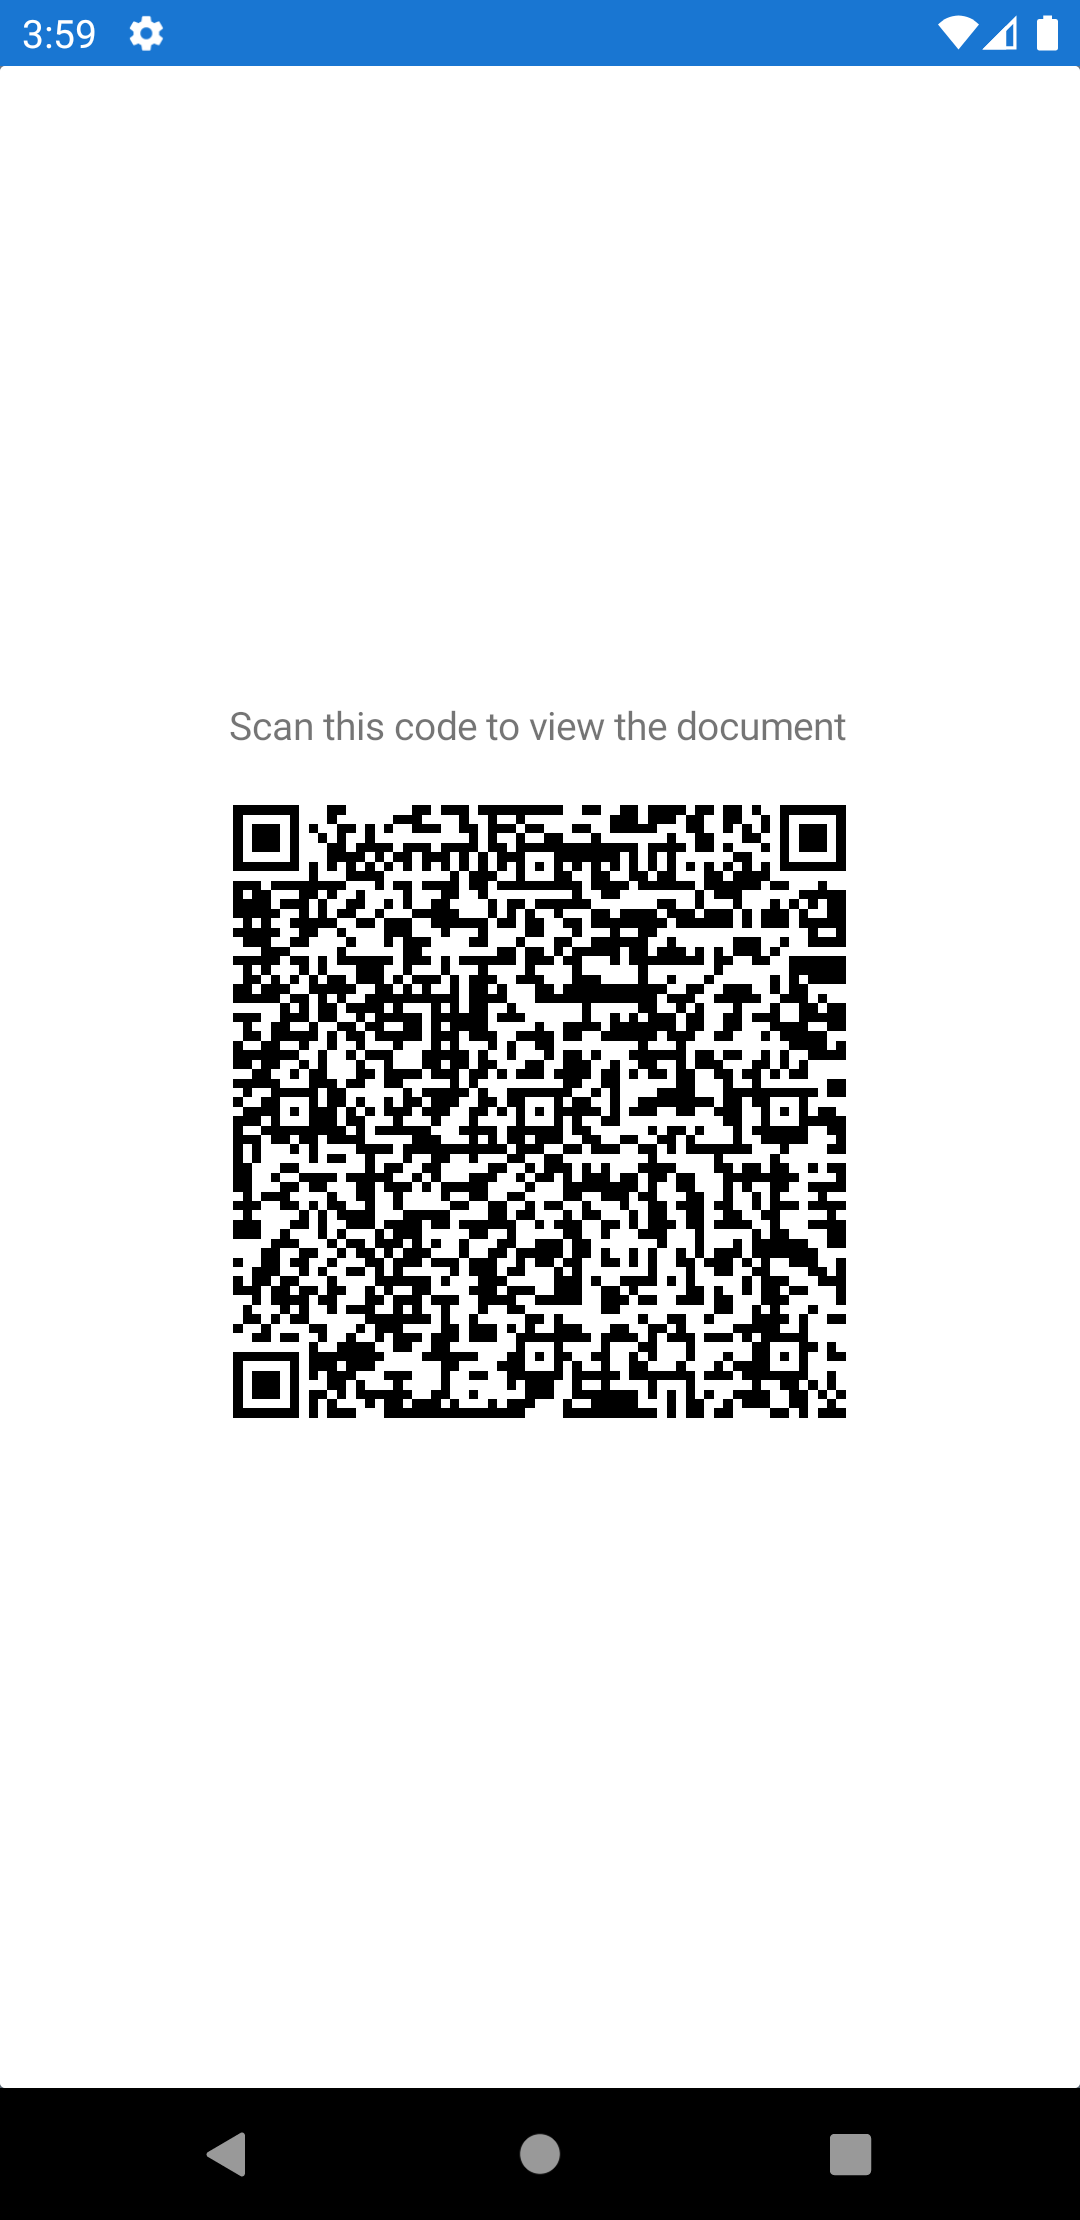
\includegraphics[scale=0.12]{share-document-page}
			\caption{Documents and Share Document pages}
		\end{figure}

		Tapping the Remove button irreversibly deletes the document from the list.
		After a successful removal the user is able to request a new document of the same type.
		If the document template was modified since
		the previous request or the user modified their personal information, the resulting document may be different than the previously deleted one.

		The Share button allows the user to safely transfer their selected document to a different device.
		Upon tapping the button, the application generates a unique code for the document which is then displayed on the screen via a QR code.

		The code can be read using the "Scan QR code" button. 
		Tapping this button will attempt to open the device's main camera in order to scan the code.
		If this feature is accessed for the first time, a prompt appears asking for the user's permission to use the camera.
		If the permission is granted, the application will open the camera app. 
		Upon successfully reading a QR code generated by E-me, the selected document will appear on the screen (see \hyperref[document]{Document Viewer}).

	\section{Requesting a Document}

	The Request Document page consists of a list of document types that can be acquired by the user.
	The list only contains types that are not yet owned by the corresponding user.
	If the user acquires one of these document types, it will disappear from the list (it will be listed on the \hyperref[documents]{My Documents} page instead).

	Combined with the \hyperref[documents]{My Documents} page, these two lists contain every document type that can be managed through the application. 
		\begin{figure}[H]
			\centering
			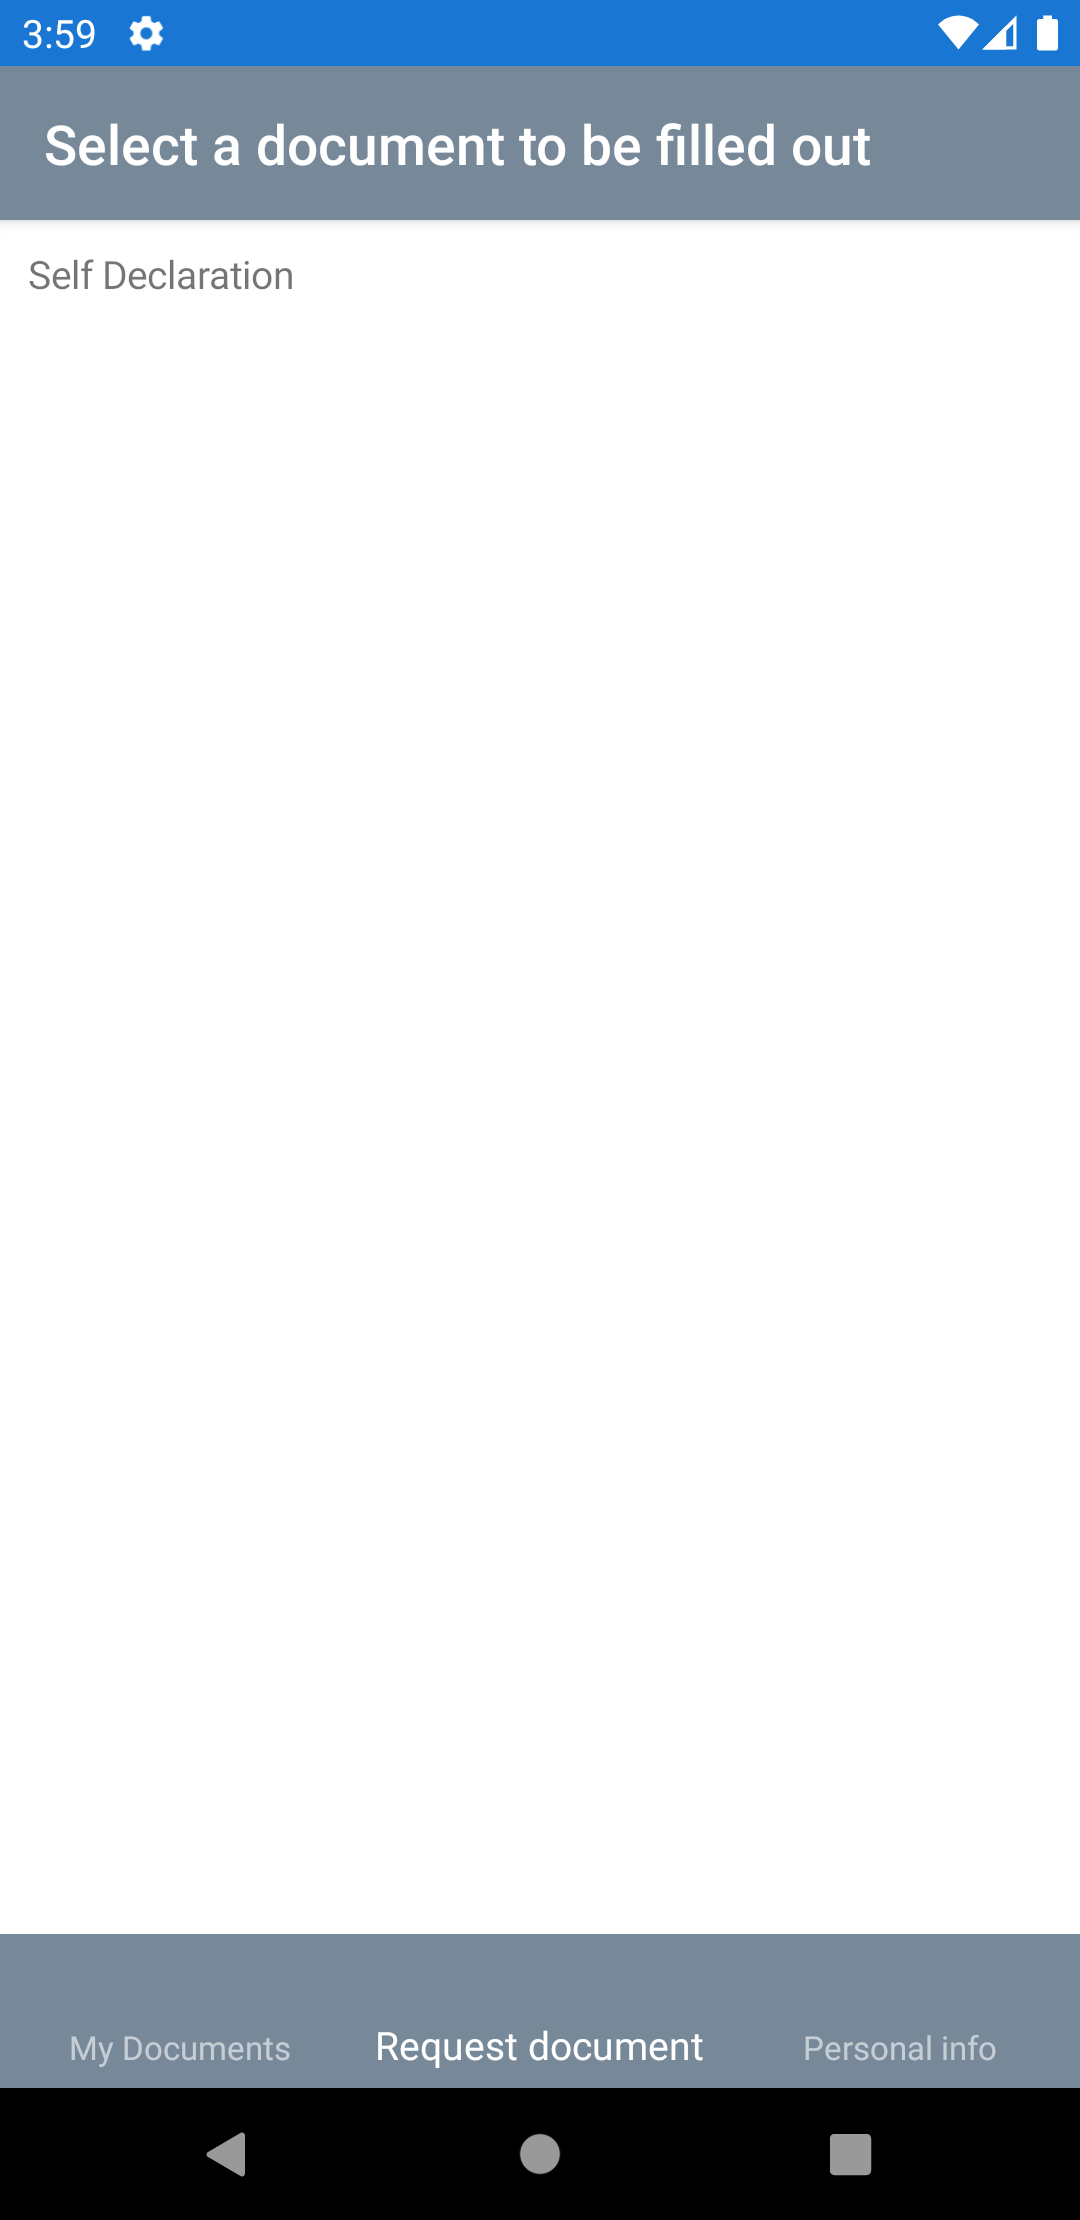
\includegraphics[scale=0.12]{request-document-page}				
			\caption{Request Document and Personal Information pages}
		\end{figure}

		The user can request a document by simply tapping on an item from the list. 
		The requested document will be generated and automatically displayed on the screen (see \hyperref[document]{Documents Page}).

	\section{Personal Information}

	This page contains several fields containing the personal details of the user. 
	Neither of these fields are required, however if no information is provided about the user, the application will not be able to automatically fill the requested documents.
	The information provided by the user on this page will be stored in an encrypted form.
		
	\begin{figure}[H]
		\centering
		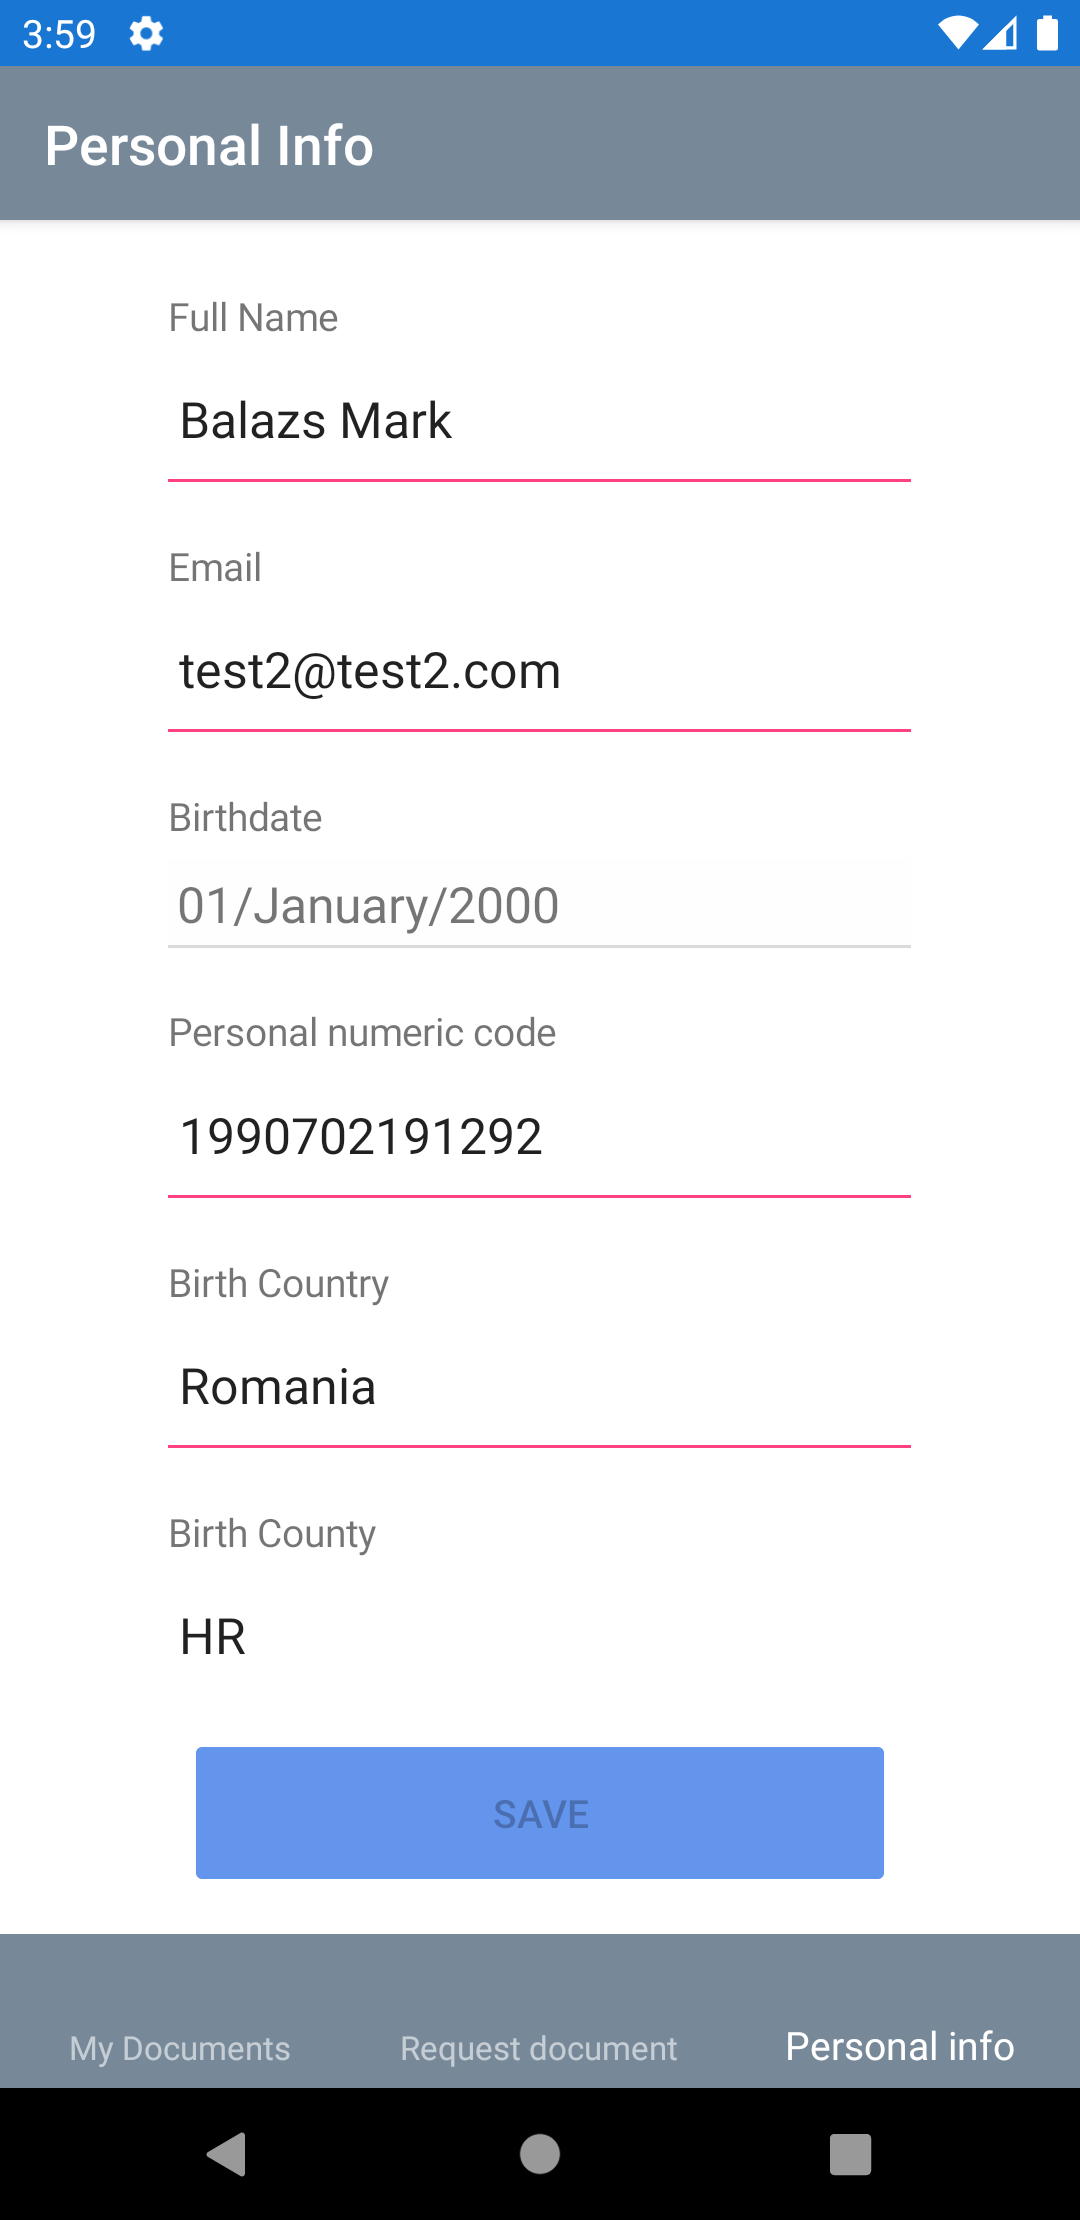
\includegraphics[scale=0.12]{personal-info-page}
		\caption{Request Document and Personal Information pages}
	\end{figure}

	Upon requesting a document, E-me attempts to match the fields of the document with the information of the user and fill them out respectively.
	Fields that require information that is not provided by the user will be left blank and can be filled manually on the \hyperref[document]{Document Viewer}.

	\section{Document Viewer}\label{document}

	On this page a PDF Viewer can be seen which allows the user to inspect or even edit their documents.
	This viewer supports text searching, bookmarking, zooming, printing and/or saving a PDF to the local storage of the mobile device.
	The contents of the PDF are generated by the application, however if the document contains fields that could not be matched with any user data,
	the user is able to fill them out manually. This page can be closed by pressing the Back button.

		\begin{figure}[H]
			\centering
			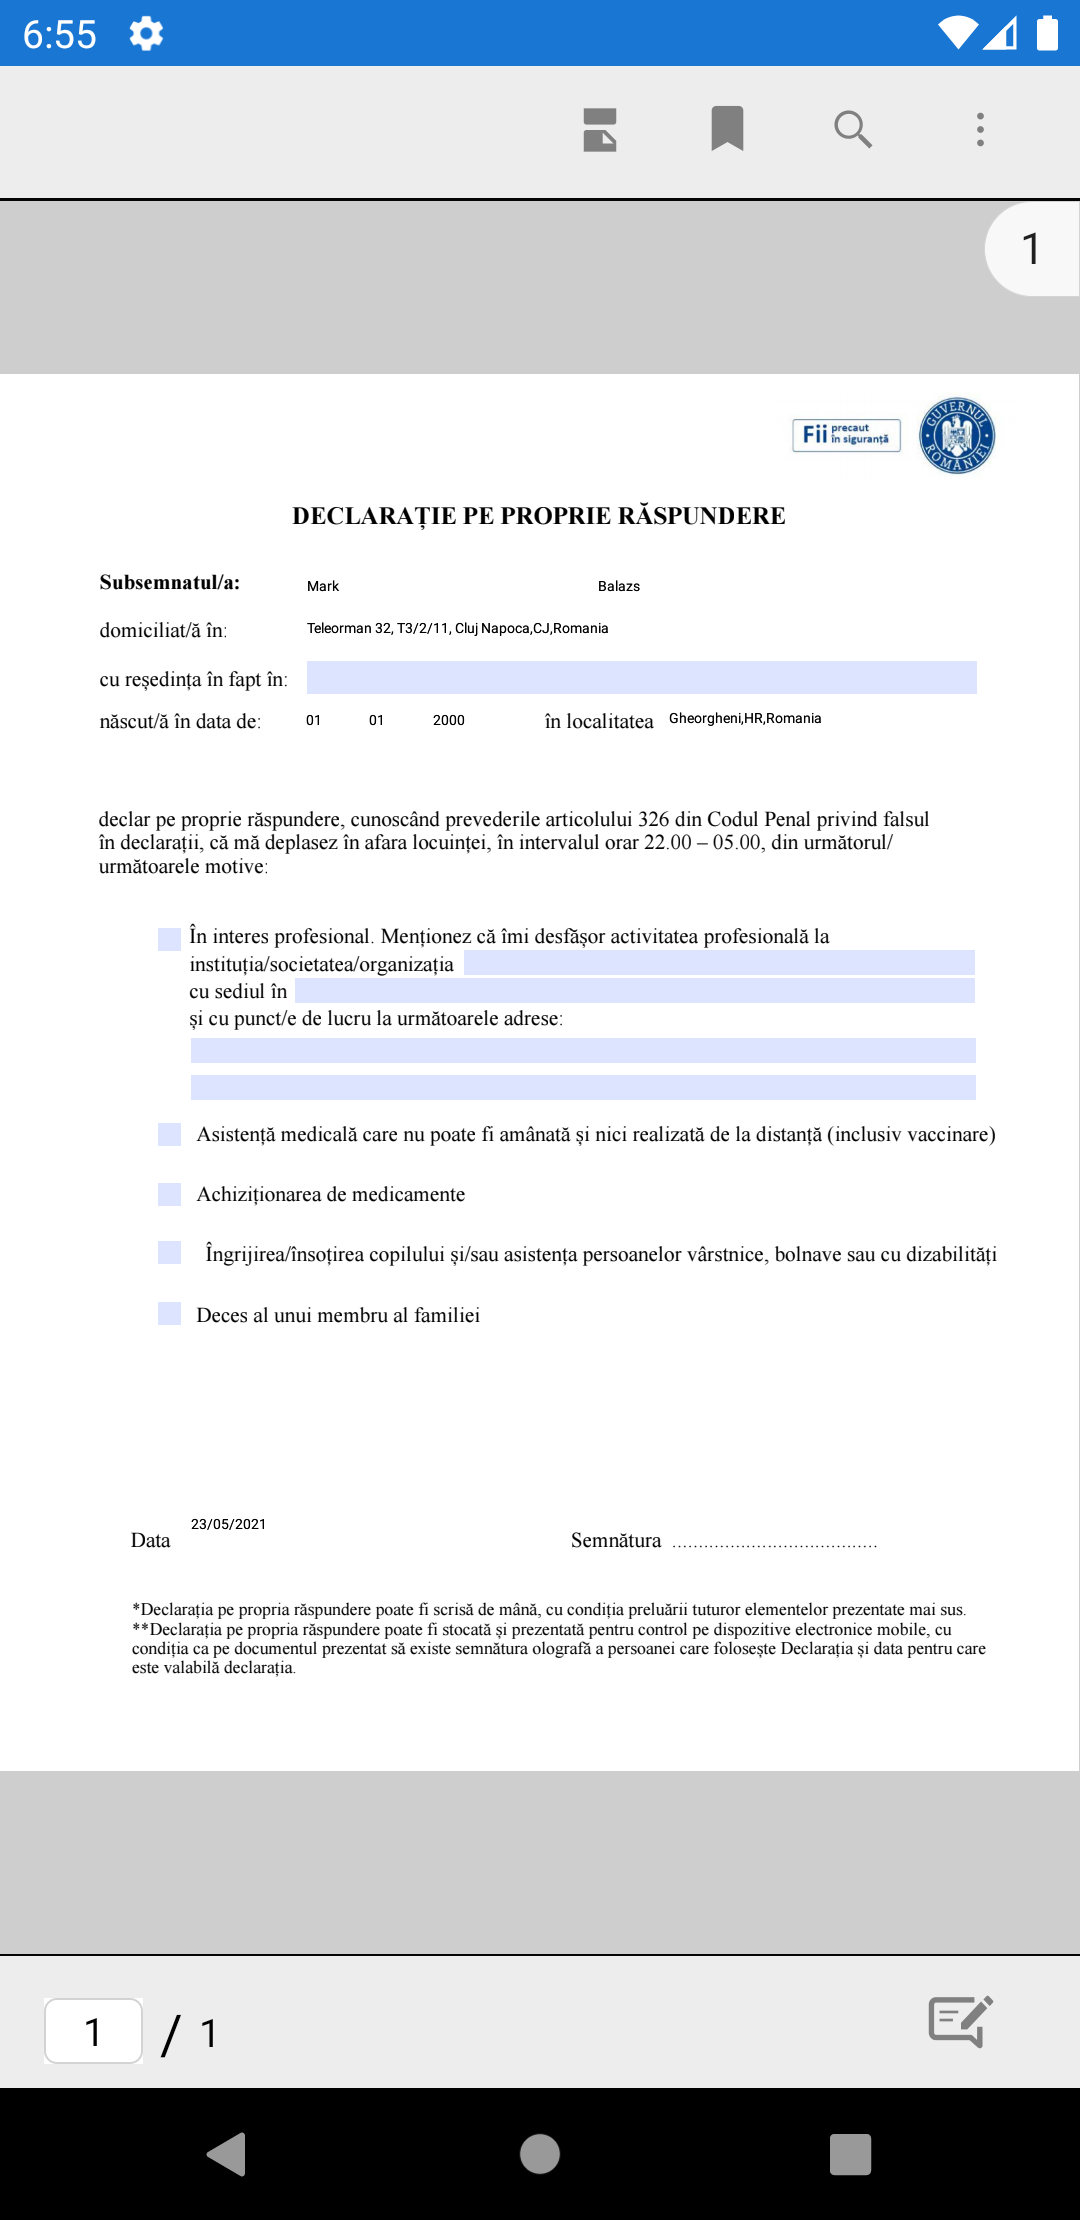
\includegraphics[scale=0.12]{document-page}
			\caption{Document Viewer}
		\end{figure}